%%%%%%%%%%%%%%%%%%%%%%%%%%%%%%%%%%%%%%%%%
% Programming/Coding Assignment
% LaTeX Template
%
% This template has been downloaded from:
% http://www.latextemplates.com
%
% Original author:
% Ted Pavlic (http://www.tedpavlic.com)
%
% Note:
% The \lipsum[#] commands throughout this template generate dummy text
% to fill the template out. These commands should all be removed when 
% writing assignment content.
%
% This template uses a Perl script as an example snippet of code, most other
% languages are also usable. Configure them in the "CODE INCLUSION 
% CONFIGURATION" section.
%
%%%%%%%%%%%%%%%%%%%%%%%%%%%%%%%%%%%%%%%%%

%----------------------------------------------------------------------------------------
%	PACKAGES AND OTHER DOCUMENT CONFIGURATIONS
%----------------------------------------------------------------------------------------

\documentclass{article}

\usepackage{fancyhdr} % Required for custom headers
\usepackage{lastpage} % Required to determine the last page for the footer
\usepackage{extramarks} % Required for headers and footers
\usepackage[usenames,dvipsnames]{color} % Required for custom colors
\usepackage{graphicx} % Required to insert images
\usepackage{listings} % Required for insertion of code
\usepackage{courier} % Required for the courier font
\usepackage{textcomp} % Required for the courier font
\usepackage{float} % for positioning pictures
\usepackage{lipsum} % Used for inserting dummy 'Lorem ipsum' text into the template

% Margins
\topmargin=-0.45in
\evensidemargin=0in
\oddsidemargin=0in
\textwidth=6.5in
\textheight=9.0in
\headsep=0.25in

\linespread{1.1} % Line spacing

% Set up the header and footer
\pagestyle{fancy}
%\chead{\hmwkClass\ (\hmwkClassInstructor\ \hmwkClassTime): \hmwkTitle} % Top center head
\rhead{\firstxmark} % Top right header
\lfoot{\lastxmark} % Bottom left footer
\cfoot{} % Bottom center footer
\rfoot{Page\ \thepage\ of\ \protect\pageref{LastPage}} % Bottom right footer
\renewcommand\headrulewidth{0.4pt} % Size of the header rule
\renewcommand\footrulewidth{0.4pt} % Size of the footer rule

\setlength\parindent{0pt} % Removes all indentation from paragraphs

%----------------------------------------------------------------------------------------
%	CODE INCLUSION CONFIGURATION
%----------------------------------------------------------------------------------------

% Creates a new command to include a perl script, the first parameter is the filename of the script (without .pl), the second parameter is the caption
\newcommand{\Javas}[2]{
\begin{itemize}
\item[]\lstinputlisting[caption=#2,label=#1]{#1.java}
\end{itemize}
}

\definecolor{MyDarkGreen}{rgb}{0.0,0.4,0.0} % This is the color used for comments
\lstloadlanguages{Java}
\lstset{language=Java,
  showspaces=false,
  showtabs=false,
  breaklines=true,
  showstringspaces=false,
  breakatwhitespace=true,
  commentstyle=\color{green},
  keywordstyle=\color{blue},
  stringstyle=\color{red},
  basicstyle=\ttfamily,
  moredelim=[il][\textcolor{grey}]{$$},
  moredelim=[is][\textcolor{grey}]{\%\%}{\%\%}
}

%----------------------------------------------------------------------------------------
%	NAME AND CLASS SECTION
%----------------------------------------------------------------------------------------

\newcommand{\hmwkTitle}{Programming Assignment\ \#2} % Assignment title
\newcommand{\hmwkDueDate}{Thursday,\ October\ 23,\ 2014} % Due date
\newcommand{\hmwkClass}{CS553\ } % Course/class
\newcommand{\hmwkClassTime}{} % Class/lecture time
\newcommand{\hmwkClassInstructor}{Ioan Raicu} % Teacher/lecturer
\newcommand{\hmwkAuthorName}{Thomas Dubucq / Tony Forlini / Virgile Landeiro} % Your name

%----------------------------------------------------------------------------------------
%	TITLE PAGE
%----------------------------------------------------------------------------------------

\title{
\vspace{2in}
\textmd{\textbf{\hmwkClass:\ \hmwkTitle}}\\
\normalsize\vspace{0.1in}\small{Due\ on\ \hmwkDueDate}\\
\vspace{0.1in}\large{\textit{\hmwkClassInstructor\ \hmwkClassTime}}
\vspace{3in}
}

\author{\textbf{\hmwkAuthorName}}
\date{} % Insert date here if you want it to appear below your name

%----------------------------------------------------------------------------------------

\begin{document}

\maketitle

%----------------------------------------------------------------------------------------
%	TABLE OF CONTENTS
%----------------------------------------------------------------------------------------

%\setcounter{tocdepth}{1} % Uncomment this line if you don't want subsections listed in the ToC

\newpage
\tableofcontents
\newpage

%----------------------------------------------------------------------------------------
%	Introduction
%----------------------------------------------------------------------------------------

% To have just one problem per page, simply put a \clearpage after each problem

\section{Introduction}
The goal of this programming assignment is to enable us to gain experience programming with:
\begin{itemize}
  \item Amazon Web Services, specifically the EC2 cloud (http://aws.amazon.com/ec2/)
  \item The Hadoop framework (http://hadoop.apache.org/)
  \item The Swift parallel programming system (http://swift-lang.org/main/)\\
\end{itemize}

Apache Hadoop is an open-source software framework for storage and large-scale processing of data-sets on clusters of commodity hardware. Hadoop is an Apache top-level project being built and used by a global community of contributors and users. It is licensed under the Apache License 2.0.

Swift is an implicitly parallel programming language that allows to write scripts that distribute program execution across distributed computing resources, including clusters, clouds, grids, and supercomputers. Swift implementations are open source under the Apache License, version 2.0.

Thomas Dubucq has developed the sorting on MPI.
Tony Forlini has developed the Hadoop wordcount. He deployed it on a virtual cluster from one node to seventeen nodes and ran the corresponding tests.
Virgile Landeiro Dos Reis has developed the shared memory wordcount and the Swift wordcount. He deployed Swift on a virtual cluster from one node to seventeen nodes and ran the corresponding tests.

\section{Set up a one node Virtual Cluster}

We set up a virtual cluster of 1 node using the Amazon EC2 Dashboard in few minutes by making a spot request of a c3.large instance using the AMI ami-3d50120d.

\begin{figure}[h!]
  \centering
  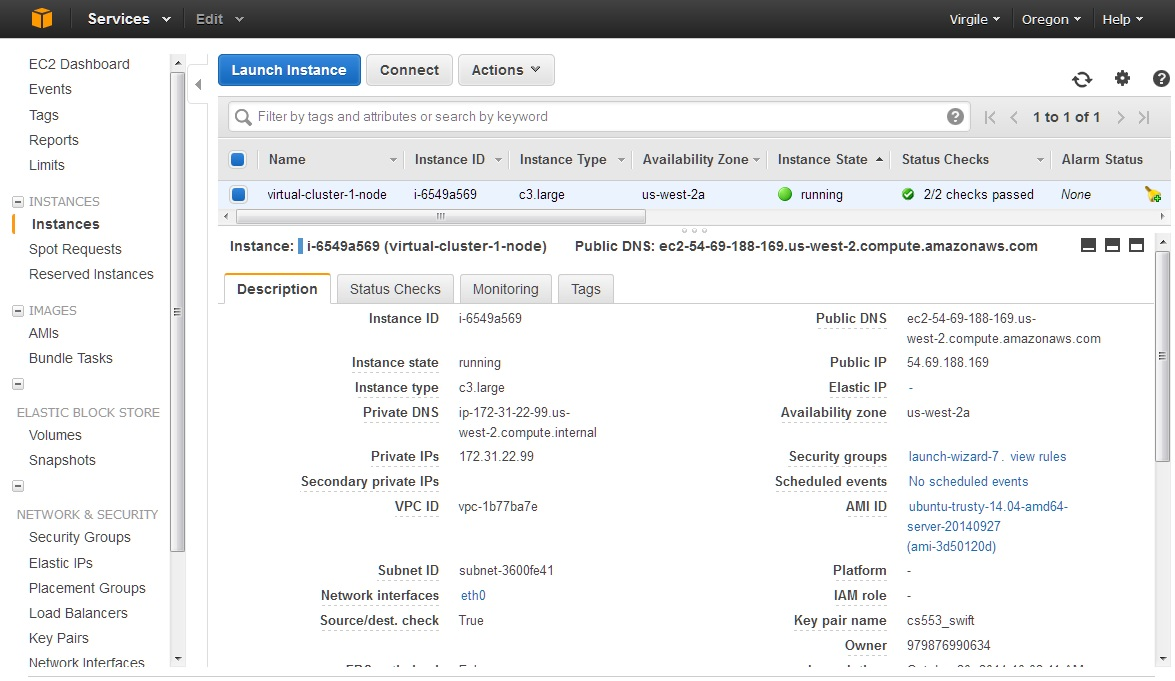
\includegraphics[width=0.9\textwidth]{img/virtual-cluster-one-node.jpg}
  \caption{Screenshot of the AWS Dashboard with one c3.large instance running.}
\end{figure}
Once the instance is running, we can choose to install Hadoop, Swift, or any tools required to run our shared memory wordcount (git, python modules, etc).


\section{Shared-Memory WordCount}

\subsection{Implementation}

We chose to implement the shared-memory WordCount in Python. To allow concurrence and get the best out of the CPU(s), we use the \lstinline|multithreading| package. The program is divided in three parts:

\begin{enumerate}
  \item{The pre-processing part splits the input files into N shards by building a queue $Q$ of $N$ pairs $(offset, size)$.}
  \item{The second part runs $T$ threads with the same process running on each thread. Each thread has access to:
    \begin{itemize}
      \item{the shared queue $Q$ of shards build in the first step;}
      \item{a shared list $R$ to store the results.}
    \end{itemize}
 The process for each thread is defined as follows: while $Q$ is not empty, the thread pops a pair $(offset, size)$ ot it, counts the words contained in the corresponding shard, and accumulate the results in a local dictionary $D$. When $Q$ is empty, $D$ is appended to the shared list $R$.}
 \item{The main program retrieves the local dictionaries from $R$ and merge them into a global dictionary to get the total counts of all the words in the input file.}
\end{enumerate}

Note that we pay attention not to cut a word in two when splitting the input file in order to get the correct words count.

\subsection{Performance Evaluation}
To find the best performance, we vary the numbers of processes from 1 to 8 on a c3.large instance with AMI ami-3d50120d and we get the results shown in Table \ref{table:python-threads-performance}

\begin{table}[h!]
  \centering
  \begin{tabular}{|c|c|}
    \hline
    \textbf{\# Threads} & \textbf{Execution time (s)} \\
    \hline
    1 & 10 min 49.149 s \\
    \hline
    2 & \textbf{9 min 50.513 s} \\
    \hline
    4 & 10 min 39.232 s \\
    \hline
    8 & 10 min 14.444 s \\
    \hline
  \end{tabular}
  \label{table:python-threads-performance}
  \caption{Performance results for the Python Wordcount}
\end{table}

We can see that the best performance is achieved when we run 2 processes at the same time. This seems to be logical as the c3.large instances have two virtual CPUs so when only one process is running, all the computing power is not used, and when more than 2 processes are running, the execution is slowed down by the fact that memory is shared between the processes.

\subsection{Bugs encountered and Fixes}

\subsubsection*{Memory Error}

\paragraph{Description: }

In the first version of the Python wordcount code, the number of shards was defined by the number of processes running, i.e. if we were running the program on 4 processes, then the input file would have been divided in 4 shards.
This was working alright until we started running the wordcount on the 10GB dataset. Indeed, if we keep the previous example, the program now divide the input file in shard of 2.5GB which is too large for the memory with other programs running.

\paragraph{Fix: }

To quickly fix this problem, we added the number of shards to create as a parameter of our Python wordcount. Therefore, the parameters of the Python wordcount program are now the number of shards to create, the number of processes to run, and the input file.

\subsubsection*{CPUs are not all used}

\paragraph{Description: }

A previous version of the code was using the class \lstinline|threading.Thread| class to create multiple threads and therefore, process multiple shards at a time. However, it appears that the \lstinline|threading| module is not able to distribute the created threads over multiple CPUs due to some Python limitations. Consequently, we were not able to see any progress in the execution time of our program when running it on multiple threads as only one CPU was used by this program.

\paragraph{Fix: }

To run our program on several CPUs, we used the \lstinline|multiprocessing| module that allows maximal use of the CPUs on a machine by implementing shared memory mechanisms.


\section{Hadoop}

\subsection{Functioning}
As we said previously, Apache Hadoop is an open source framework for cloud computing, and more precisely for storage and large scale processing on commodity clusters. Hadoop is an alternative to the Google Mapreduce framework. Hadoop allows to distribute Map reduce jobs on several workers nodes which are handled by one or more master node. Hadoop is made of the following components:

\begin{itemize}
  \item HDFS is the Hadoop distributed file system that is responsible for the storage of data. It is composed by a NameNode on the master which holds all the metadata regarding the stored files and manages the file system namespace and regulates access to files by clients and DataNodes on the workers which contain actual data and manage storage attached to the nodes that they run on.
  \item YARN is Apache Hadoop NextGen MapReduce that is responsible for resource management and job scheduling/monitoring. It is composed by a ResourceManager on the master which is responsible for allocating resources to the various running applications and accepting job-submissions. On the other side , the NodeManager  is the per-machine framework agent who is responsible for containers and monitoring resource usage.
\end{itemize}

\begin{figure}[!ht]
   \centering
   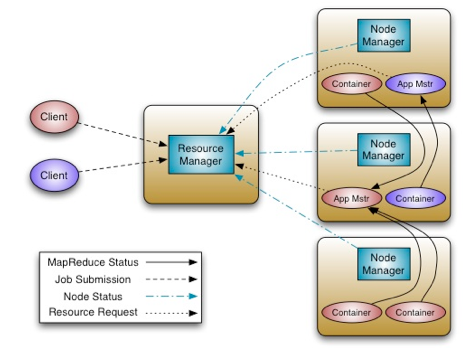
\includegraphics[width=0.45\textwidth]{YARNArch.png}
   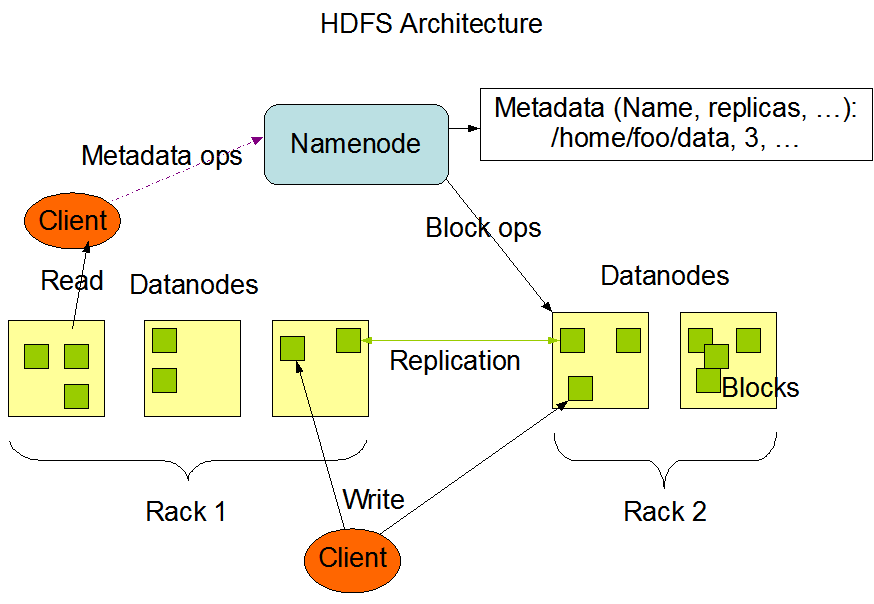
\includegraphics[width=0.45\textwidth]{hdfsarchitecture.png}
\caption{HDFS and YARN Architectures}
\end{figure}


\subsection{Installation}

This assignment requires to setup a cluster of 17 nodes with hadoop installed on it. We need to separates setups for the master node and the workers. The setup can be done for one worker and then replicated using an AMI. We made a bash script to automate the installation.

First we install the Master. We need to install a Java virtual machine on all the node, which is used to run hadoop. We chose the Java-7-openjdk version. Then we chose to install Hadoop v2.4.0 which is fairly recent and using YARN rather than former MapReduce on legacy versions of Hadoop. Then we need to configure the environment variables for hadoop.

We also need to setup ssh connexion between the master and the workers so that they can connect automatically without password. To do so we use a RSA key authentication in which the master provides its public key to all the workers. This will allow hadoop scripts to launch automatically the HDFS and YARN daemons on all the nodes.

Then we need to setup the HDFS configuration. There are two configuration files which are called hdfs-site.xml and core-site.xml. The first one specifies the path to the local filesystem for both the NameNode and the DataNodes. The second one holds the domain name of the NameNode so that the hadoop modules know where the NameNode is.

Second we configure YARN using the yarn-site.xml configuration file. In this file we setup the resource allocation of hardware according to our machines. As we will run our Worcount on c3 large instances, we chose a maximum memory for each scheduler to 2048 MB, 1 virtual cores per container, 2 virtual cores per scheduler and 4096MB of memory for the NodeManager.

Finally we need to format the namenode to the hadoop file system. Once it’s done we can start the HDFS and YARN daemons on the master. Assuming the Workers are already configured, we can add their domain name to the slave’s file of the master. It will allow hadoop to run all the daemons on all the node at the same time.

We need now to configure the workers. As for the master we install Java and download the same version of hadoop. We also setup the environment variables as previously. Then we configure the hdfs-site.xml file by setting the domain name of the machine running the NameNode daemon ie. the master. To configure YARN we modify the yarn-site.xml by adding the domain name of the ResourceManager ie. the master.

\subsection{Issues}

We had some troubles launching the WordCount job on a cluster of 17 nodes with m3.large instances (c3.larges weren't available for 17 nodes clusters ans AWS refused us the access). With the 1MB dataset, The Worcount works perferctly (even with a 270MB or 1GB dataset input), but when we ran the Word count with a 10GB input, the map task was rather slow and stopped at 40\% saying that all the space on the disk was used although we added EBS partitions to the HDFS storage. We assume that the m3.large instances are not designed to that kind of computation which implies high disk utilisation. Thus the results we obtained for the Hadoopword count are based on a 1GB input.

\subsection{WordCount Implementation}

The map class reads the input line by line, and separate each line into words according to a separator (here space " " ). The word is called a token. Then the map function returns a pair of key, value which is (token,1).

\Javas{wordcount}{Map function}
The reduce function gets the shuffled key,vlue pairs and just sums the number of value in the list of each token.

\Javas{new2}{Reduce Function}

The run method allows to setup some configuration for the job, such as the input/output paths, key/value types or input/output formats.

\Javas{new3}{Run Function}

\subsection{Configuration Files}

Once we implemented the wordcount, we need to compile it with the hadoop-commons library and then create a jar file. But the cluster has to be configured a different way according the number of slave on which we intent to run the job. Thus the conf/master is supposed to specifiy the master's address, but this file exist only on former versions of Haddop (1.x.x). The conf/slaves specifies the slaves adresses so that the master can automatically connect with the workers. the conf/core-site file specifies the NameNode address.\\

The conf/hdfs-site specifies the path on the local filesystem of a DataNode where it should store its blocks, and Path on the local filesystem where the NameNode stores the metadata. Finally the conf/mapred-site specifies parameters such as the number of core required for each task, the memory allocated for map and reduce tasks or the heap size for jvm childs.

All of the configuration files must include port numbers when it refers to the master domain name URI because these ports are used by Hadoop’s daemons to communicate amongst themselves (to schedule jobs, replicate blocks, etc.). So if those ports are not fixed two daemons may use the same port leading to the fact that one daemon will be blocked. We can change the numbers of mapers and reducers from the configuration files by adding cores and memory to containers. 


\section{Swift}

\subsection{Installation}

For this assignment, we used Swift 0.95 with Java 7 from the OpenJDK distribution.

\subsubsection*{One node cluster}

Installing Swift on a one node cluster is relatively easy as an archive with an installation script included is given. Once an AWS instance is running, we need to install java on it if it is not already done, extract the archive, and run the installation script to get a running installation of Swift.

\begin{figure}[!ht]
   \centering
   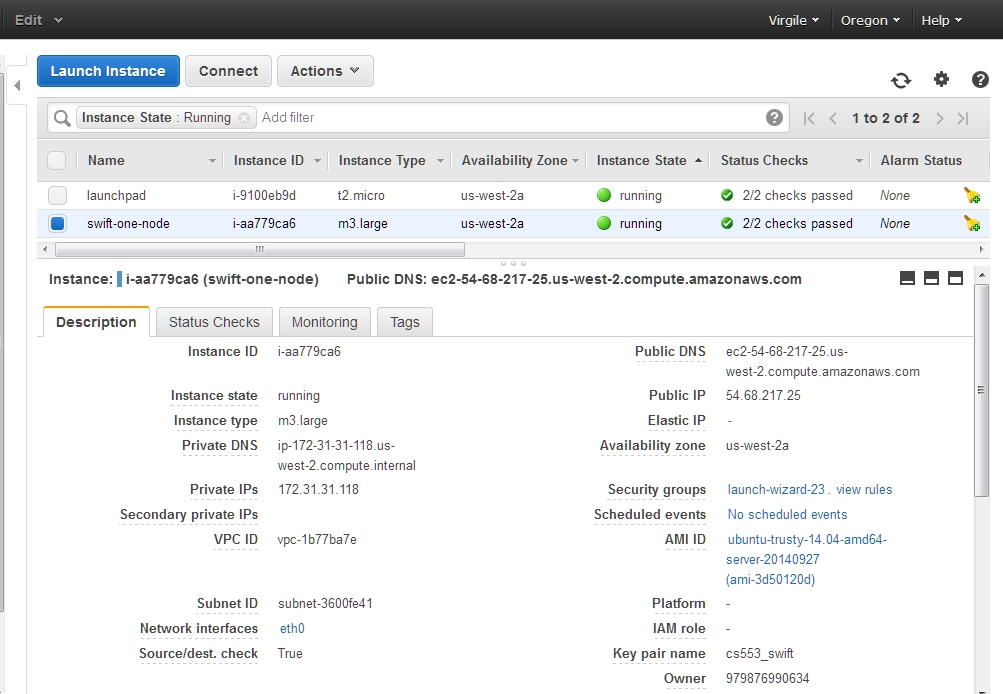
\includegraphics[width=0.45\textwidth]{img/swift-one-node.jpg}
   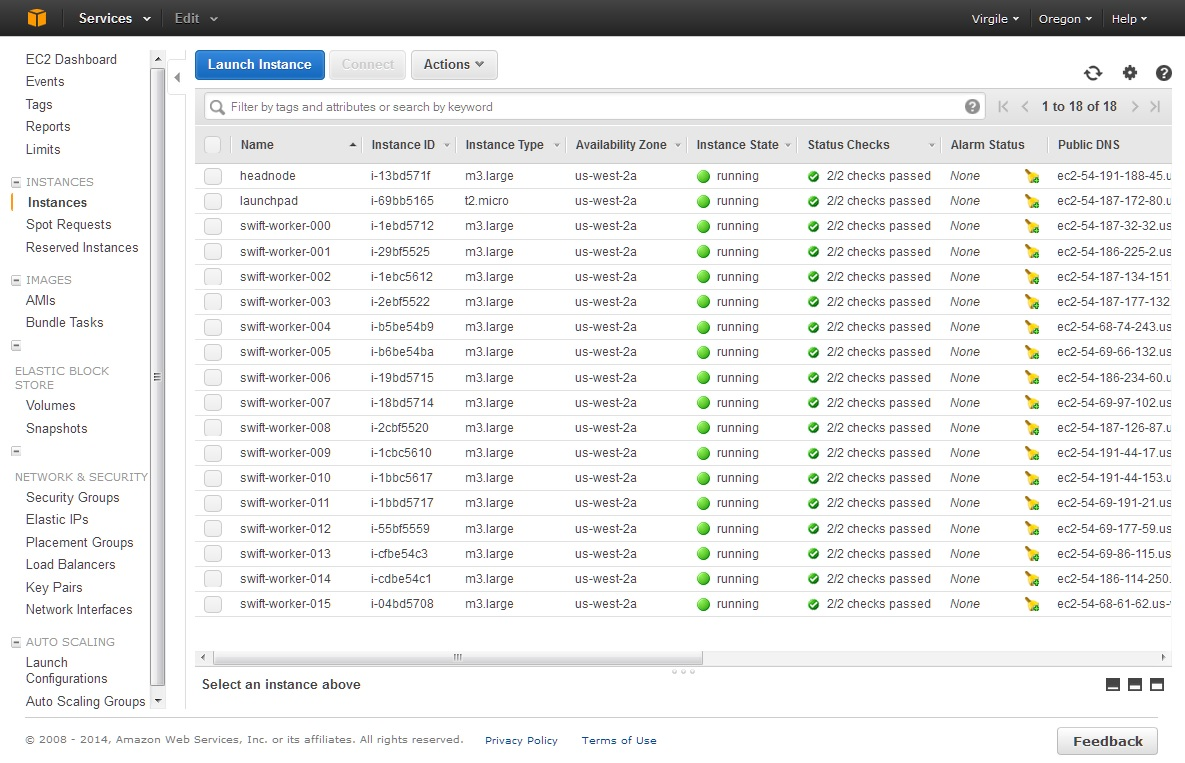
\includegraphics[width=0.45\textwidth]{img/swift-n-nodes.jpg}
\caption{Swift running on a one node virtual cluster (left) and on a seventeen nodes virtual cluster (right).}
\end{figure}

\subsubsection*{Multiple nodes cluster}

To install Swift on a multiple nodes cluster, more work than just extracting files from an archive is required.

First, we need to create an IAM User and give it the Administrators right.
Then we need to modify some configuration files to manage the cloud resources but also to manage the jobs distribution over the workers.

To manage the cloud resources, we change the following values in \lstinline|cloud-tutorials/ec2/configs|:

\begin{lstlisting}
AWS_CREDENTIALS_FILE=$HOME/cs553-cloudcomputing-2014/assignment2/conf/swift/credentials.csv
AWS_WORKER_COUNT=2
AWS_KEYPAIR_NAME=node
AWS_KEYPAIR_FILE=$HOME/cs553-cloudcomputing-2014/assignment2/conf/node.pem
HEADNODE_MACHINE_TYPE=m3.large
WORKER_MACHINE_TYPE=m3.large
\end{lstlisting}

The credentials file is related to the IAM User we created in the first step. We also create a pem key file to be able to connect to the headnode and to the workers.

To manage the jobs distribution, we need to change the file \lstinline|swift.conf| in our development directory:

\begin{lstlisting}
sites: cloud-static

site.local {
    filesystem {
        type: "local"
        URL: "localhost"
    }
    execution {
        type: "local"
        URL: "localhost"
    }
    workDirectory: /tmp/${env.USER}/swiftwork
    maxParallelTasks: 32
    initialParallelTasks: 31
    app.ALL {executable: "*"}
}

site.cloud-static {
    execution {
        type:"coaster-persistent"
        URL: "http://127.0.0.1:50010"
        jobManager: "local:local"
        options {
            maxJobs: 32
            tasksPerNode: 2
        }
    }

    initialParallelTasks: 20
    maxParallelTasks: 20
    filesystem.type: local
    workDirectory: /tmp/swiftwork
    staging: local
    app.ALL {executable: "*"}

}

lazyErrors: false
executionRetries: 0
keepSiteDir: true
providerStagingPinSwiftFiles: false
alwaysTransferWrapperLog: true
\end{lstlisting}

The first line \lstinline|sites| is set to \lstinline|local| when we want to run a Swift script on one node which will be master and worker at the same time. When we want to run our script on a cluster, \lstinline|sites|' value is \lstinline|cloud-static|. Moreover we set the value of site.cloud-static.execution.options.tasksPerNode to 2 because each worker node will have two virtual CPUs to run tasks.

\subsection{WordCount Implementation}

The Swift implementation of the WordCount is similar to the Hadoop and Python implementations because we procede in three steps:

\begin{enumerate}
  \item The input data is split in a finite number of shards. When starting the development of the Swift script, we wanted to integrate the input split in it but as Swift is optimized for parallel, it is difficult to force such a script to perform a sequential task. Therefore, it is easier to implement a split out of the Swift script and then run the Swift script on the generated shards. We use \lstinline|split| to create the shards and store them in the folder \lstinline|/data/inputs/|:\\
  \lstinline|split -n l/$NSHARDS -d $DATASET /data/inputs/d_ --additional-suffix=".shard"|. One again, we pay attention not to split a word in two when creating the shards.
  \item The shards are distributed over the workers and each worker perform a WordCount task over the shards it receives. First, we map each shard to a unique variable in Swift using a \lstinline|single_file_mapper|. Then, in order to distribute the shards to the workers, we use the \lstinline|foreach| loop in the Swift script. This instruction automatically distributes each iteration of the loop to a different worker. In our code, the content of the loop consists of running a wordcount built with \lstinline|tr|, \lstinline|sort|, and \lstinline|uniq| commands:\\
  \lstinline£cat $1 | tr -d ",;.|'" | tr " \t\v\b" "\n" | tr -s "\n" | sort | uniq -c£. Each output file is mapped to a Swift variable and stored into an array.
  \item The temporary word counts are merged by the master node into a global wordcount. This is done using the same method as the \lstinline|cloud-cat| provided in the Swift tutorial except that instead of doing a simple cat, we sum the counts for words that are the same using \lstinline|sed| and \lstinline|awk|. Moreover, we sort the global output in descending frequency order using \lstinline|sort|:\\
  \lstinline£cat $*| sed 's/^[[:blank:]]*//;s/[[:blank:]]*$//' | awk -F " " \ £\\
  \lstinline£'{arr[$2] += $1} END {for (i in arr) { print arr[i], i}}' | sort -nr | less£
\end{enumerate}

\subsection{Performance Evaluation}

To evaluate the performance, we vary the numbers of workers from 1 to 16 on a m3.large instance and we get the results shown in Table \ref{table:swift-threads-performance}

\begin{table}[h!]
  \centering
  \begin{tabular}{|c|c|}
    \hline
    \textbf{\# Worker} & \textbf{Execution time} \\
    \hline
    1 & 58 min 13 s \\
    \hline
    2 & 13 min 48 s \\
    \hline
    4 & 8 min 30 s \\
    \hline
    8 & 6 min 40 s \\
    \hline
    16 & 6 min 6 s \\
    \hline
  \end{tabular}
  \label{table:swift-threads-performance}
  \caption{Performance results for the Swift Wordcount}
\end{table}

Let us note that we have timed the shards creation and it takes approximately three minutes. Therefore, it should be possible to improve the total times by reducing this time of shards' creation.
Moreover, the command line functions are probably not the best tools to operate on integer when merging the wordcount files

\subsection{Bugs encountered and Fixes}

\subsubsection*{Impossible to run 17 c3.large instance simultaneously}
\paragraph{Description: } Amazon impose a limit of 5 c3.large on demand instances for new users of AWS. We have made a request to increase this limit but it has been denied by the customer service.
\paragraph{Fix: } We ran the benchmarks on m3.large instances.

\section{Performance}

Considering our results, we have only been able to draw the execution time graphs for the shared memory wordcount (Python) and for the Swift wordcount.

We can observe that the shared memory version is faster than any distributed version when running the program on only one node (up to 6 times faster). However, when running on several nodes, Swift clearly takes advantage of the work distribution as the execution time for the same job decreases from 58 minutes on one node to approximately 6 minutes on 16 nodes.

\begin{figure}[!ht]
   \centering
   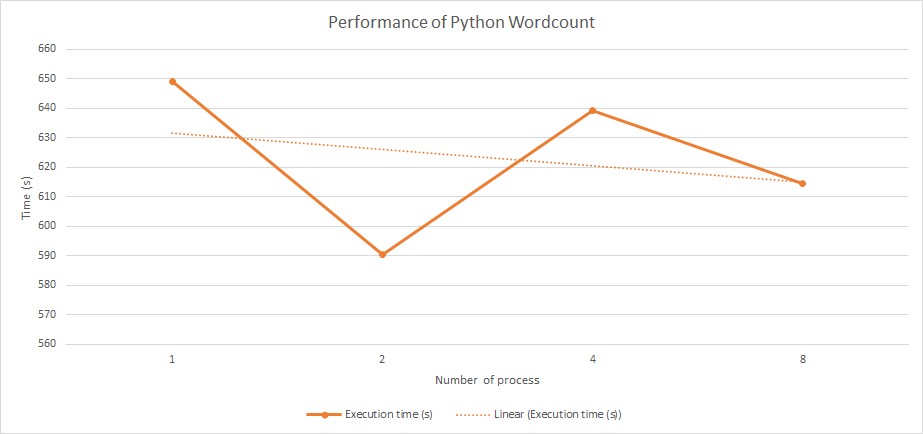
\includegraphics[width=0.45\textwidth]{img/perf-python.png} 
   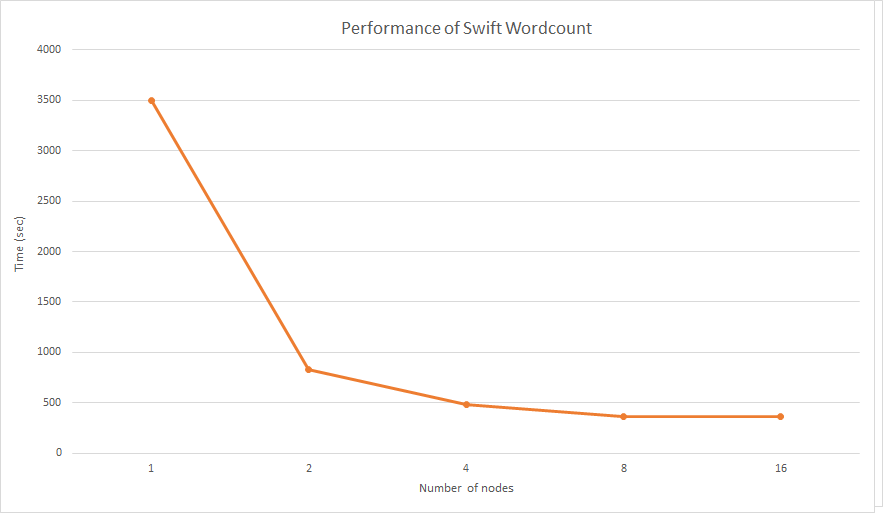
\includegraphics[width=0.45\textwidth]{img/perf-swift.png}
  \caption{Execution time for the Python wordcount in function of the number of process (left) and for the Swift wordcount in function of the number of workers.}
\end{figure}

\begin{figure}[!ht]
   \centering
   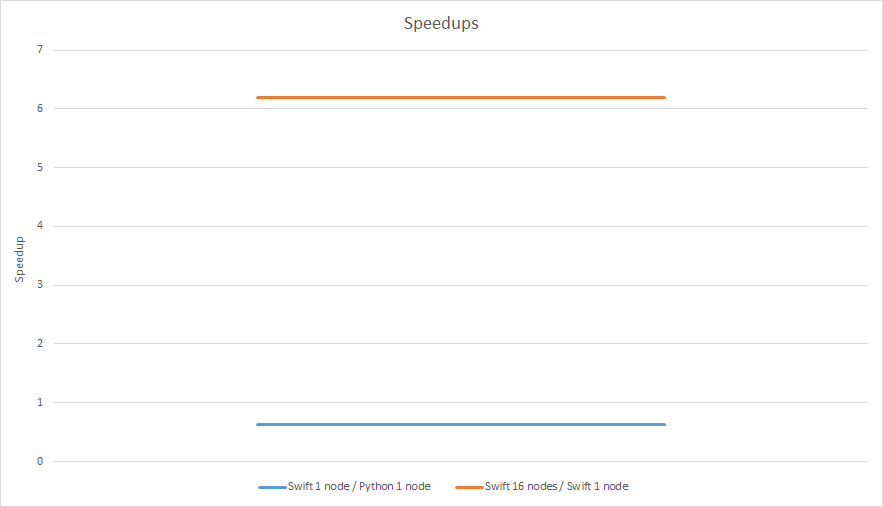
\includegraphics[width=0.95\textwidth]{img/speedup.png} 
  \caption{Speedups for Swift (one node) relative to Python and for Swift (16 nodes) relative to Swift (one node).}
\end{figure}

\section{Sort on Shared-Memory, Hadoop, Swift, and MPI}

\subsection{Sort on MPI}

Message Passing Interface (MPI) is a standard describing interaction between processes. It is specially designed to be used on large, scalable parallel applications. In this part of the assignment, the C openmpi library was used. This library allows to launch a single application on multiple processes/nodes and manages the communication details between them.

\paragraph{Program conception explanation}

In this part, we will try to justify  the conception choices made to develop a sorting program with the MPI library.

The are several task to execute in this problem : sort shards, merge sorted shards, hand out shards to the different nodes and gather results. Sorting and merging will be worker’s job while distributing shards and gathering the final result will be a responsibility given to a single master node.

The temporal distribution of jobs among workers is a difficult subject. The easiest method is to assign every worker to the sorting task and then merge the sorted elements. We chose not to follow this idea since in my opinion, the network usage is really bursty with this approach and that could cause congestion and delay the execution progress.

Our approach is as follow: all nodes are assigned to sort a first shard. Then, a subset of the workers are assigned to merging while the others are given new shards to sort. The sorting node send their result to the merger and get a new shard from the master until there is no shard left. Then, the merging nodes gather the last sorted shard and start to send their accumulated data to each other, until all the data is in a single node, that will then send it back to the master.

The sorting is made by using a quick sort algorithm and the merging is inspired from the merging part of the merge sort algorithm.

Currently the program is meant to sort integers, but the transition to character strings is not that much of a problem. Unfortunately a segmentation fault arose during the local debugging. This segmentation fault occurs in a MPI function (''Program received signal SIGSEGV, Segmentation fault. \_\_memmove\_ssse3\_back() at ../sysdeps/x86\_64/multiarch/ memcpy-ssse3-back.S:131   131     ../sysdeps/x86\_64/multiarch/ memcpy-ssse3-back.S: No such file or directory'') This error is sparsely documented, but none of the few solutions found on the net worked.

\newpage

\title{\vspace{2in}
\LARGE
\textmd{\textbf{Sources}\\
}
\normalsize
\begin{itemize}
\item http://www.itp.phys.ethz.ch/education/hs12/programming\_techniques/openmpi.pdf
\item http://www.open-mpi.org/doc/v1.8/
\item http://www.lam-mpi.org/tutorials/one-step/ezstart.php
\item http://mpitutorial.com/mpi-hello-world/
\item http://mpitutorial.com/dynamic-receiving-with-mpi-probe-and-mpi-status/
\item http://hadoop.apache.org/docs/current/hadoop-yarn/hadoop-yarn-site/YARN.html
\item http://hadoop.apache.org/
\item http://www.alexjf.net/blog/distributed-systems/hadoop-yarn-installation-definitive-guide/
\item http://swift-lang.org/docs/index.php
\item https://github.com/yadudoc/cloud-tutorials
\end{itemize}
\end{document}
